% =====================================================================
% X-Fusion: MIKE 2026 Final Submission
% Springer LNCS/LNAI format — Anonymous review manuscript
% Compile: pdfLaTeX → BibTeX → pdfLaTeX → pdfLaTeX
% Requires: llncs.cls, splncs04.bst, newtxtext/newtxmath, tikz, booktabs
% =====================================================================
\documentclass[runningheads,a4paper]{llncs}
\usepackage[T1]{fontenc}
\usepackage{newtxtext}
\usepackage[varvw]{newtxmath}
\usepackage{graphicx}
\usepackage{amsmath}
\usepackage{booktabs}
\usepackage{multirow}
\usepackage{tikz}
\usetikzlibrary{arrows.meta,positioning,calc}
\usepackage[hidelinks]{hyperref}
\hypersetup{%
  pdftitle={X-Fusion: Tri-Modal Transformer Fusion for Multi-Label Chest X-ray Analysis with Evaluation Integrity Analysis},
  pdfauthor={},
  pdfsubject={Anonymous review manuscript — MIKE 2026},
  pdfkeywords={multimodal learning, chest radiography, transformer fusion, evaluation leakage, reproducibility}
}

\begin{document}

\title{X-Fusion: Tri-Modal Transformer Fusion for\\Multi-Label Chest X-ray Analysis\\with Evaluation Integrity Analysis}
\titlerunning{X-Fusion: Tri-Modal Chest X-ray Analysis}
\author{K.~Vishal Reddy\inst{1} \and P.~Deepesh Reddy\inst{1} \and R.~Vignesh\inst{1} \and R.~Sidhardh Reddy\inst{1} \and Saharsh Machendra\inst{1} \and Vura Surya Venkat\inst{1}}
\authorrunning{K.~Vishal Reddy et al.}
\institute{Department of Computer Science and Engineering,\\Keshav Memorial Institute of Technology, Hyderabad, Telangana, India\\
\email{rvignesh72007@gmail.com}}
\maketitle

% =================================================================
% ABSTRACT
% =================================================================
\begin{abstract}
Multi-label chest radiograph analysis benefits from integrating visual, textual, and structured clinical data, yet most existing systems evaluate multimodal fusion without verifying the independence of auxiliary inputs from target labels.
We present X-Fusion, a tri-modal Transformer architecture that fuses BiomedCLIP image representations, CXR-BERT clinical-text embeddings, and six structured patient attributes in a shared 512-dimensional space through a learned classification token.
Training combines Asymmetric Loss with image--text contrastive alignment for fourteen thoracic findings on patient-disjoint ChestX-ray14 subsets.
We contribute three results: (i)~a compact, reproducible multimodal architecture with an inference web interface exposing visual attention and metadata attribution; (ii)~a systematic diagnosis showing that label-conditioned auxiliary inputs (generated notes and synthetic vital signs) inflate evaluation scores and invalidate clinical-performance claims; and (iii)~a new independent-input reference experiment using only real image pixels and recorded demographics, with validation-selected hyperparameters and complete per-case prediction archives.
The independent reference achieves macro AUROC 0.634 on 7{,}100 test images using logistic regression on 16$\times$16 pixels and age/sex, establishing a reproducible lower bound.
Our analysis demonstrates that evaluation integrity verification is essential before multimodal medical AI systems can claim clinical benefit.

\keywords{Chest radiography \and Multimodal learning \and Transformer fusion \and Evaluation integrity \and Reproducibility}
\end{abstract}

% =================================================================
% 1. INTRODUCTION
% =================================================================
\section{Introduction}

Chest radiography remains the most frequently performed diagnostic imaging examination worldwide, with a single radiograph potentially exhibiting multiple coexisting thoracic abnormalities~\cite{wang2017}.
Multi-label classification, where each image may receive several non-exclusive disease labels simultaneously, better reflects clinical reality than mutually exclusive single-diagnosis prediction.
NIH ChestX-ray14 provides a widely adopted benchmark containing 112{,}120 frontal-view radiographs with fourteen pathology labels~\cite{wang2017,nihdataset}.

Clinical decision-making relies not only on the radiographic image but also on patient history, vital signs, and laboratory findings.
Multimodal fusion architectures that combine imaging with structured and unstructured clinical data have therefore attracted growing research interest~\cite{biomedclip2023,cxrbert2022}.
However, a critical but often overlooked requirement is that auxiliary inputs must be \emph{collected independently} of the reference diagnosis; otherwise, the evaluation conflates input information with target leakage.

We present X-Fusion, a tri-modal Transformer prototype that integrates radiographic, textual, and structured patient information for fourteen-label chest X-ray analysis.
Beyond the architectural contribution, this paper makes three distinct contributions:

\begin{enumerate}
\item \textbf{Architecture and implementation.}
A compact four-token fusion mechanism that combines pretrained BiomedCLIP visual features, projected CXR-BERT text representations, and an MLP-encoded metadata vector through a two-layer, eight-head Transformer encoder.
An end-to-end web interface exposes predictions alongside visual attention overlays and metadata attribution views.

\item \textbf{Evaluation integrity analysis.}
A systematic diagnosis of target leakage in the evaluation pipeline: the dataset generates clinical notes from disease labels and samples vital signs conditional on disease presence.
We demonstrate that patient-disjoint splitting cannot remedy this within-case dependency and that the resulting near-perfect scores (macro AUROC $\approx$~1.0) characterize the leakage pathway rather than clinical discrimination.

\item \textbf{Independent-input reference experiment.}
New reference models trained exclusively on real image pixels and recorded demographics (age, sex), with no access to generated notes, synthetic vitals, or the original checkpoint.
These provide reproducible baselines with complete experimental archives including per-case predictions, split manifests, and software version records.
\end{enumerate}

The paper is organized as follows. Section~2 reviews related work. Section~3 describes the architecture and training methodology. Section~4 details the dataset and experimental setup. Section~5 presents the artifact reanalysis, independent baselines, and discussion. Section~6 addresses limitations and future directions. Section~7 concludes.

% =================================================================
% 2. RELATED WORK
% =================================================================
\section{Related Work}

\textbf{Chest radiograph benchmarks.}
Wang et al.\ introduced ChestX-ray14 with weakly supervised labels extracted from radiology reports~\cite{wang2017}.
CheXpert addressed uncertain labels through expert comparison and demonstrated the impact of label uncertainty on model evaluation~\cite{irvin2019}.
Both benchmarks use image-level labels without paired clinical context, making auxiliary-input integrity a concern for multimodal extensions.

\textbf{Vision Transformers in medical imaging.}
The Transformer architecture~\cite{vaswani2017} was adapted for image classification by Dosovitskiy et al.~\cite{dosovitskiy2021}.
DAViT applied domain-adapted Transformers for single-disease pneumonia detection~\cite{davit2025}.
Our work extends this paradigm to multi-label, multimodal fusion.

\textbf{Pretrained biomedical encoders.}
BiomedCLIP learns joint visual--textual representations from 15 million biomedical image--text pairs~\cite{biomedclip2023}.
CXR-BERT specializes BERT for radiology text understanding~\cite{cxrbert2022}.
X-Fusion uses both encoders as frozen or partially trainable feature extractors, projecting their outputs into a shared embedding space.

\textbf{Training objectives for imbalanced multi-label tasks.}
Asymmetric Loss~\cite{ridnik2021} down-weights easy negatives through asymmetric probability margins, addressing severe class imbalance in multi-label settings.
InfoNCE~\cite{oord2018} enables contrastive alignment between paired modalities.

\textbf{Explainability methods.}
SHAP~\cite{lundberg2017} provides model-agnostic feature attribution.
Chefer et al.~\cite{chefer2021} showed that raw attention weights alone do not constitute validated relevance or localization evidence.

% =================================================================
% 3. PROPOSED ARCHITECTURE AND METHODOLOGY
% =================================================================
\section{Proposed Architecture and Methodology}

\subsection{Modality-Specific Encoders}

Given an RGB radiograph $I$, a tokenized clinical note $T$, and an ordered metadata vector $m\in\mathbb{R}^{6}$, three modality-specific encoders produce aligned 512-dimensional representations:

\begin{align}
z_v &= f_v(I)\in\mathbb{R}^{512},
\label{eq:vision}\\
z_t &= W_t\, h_t(T)+b_t\in\mathbb{R}^{512},
\label{eq:text}\\
u &= \operatorname{Dropout}_{0.1}
(\operatorname{GELU}(W_1 m+b_1)),
\label{eq:meta1}\\
z_m &= \operatorname{GELU}(W_2 u+b_2)
\in\mathbb{R}^{512}.
\label{eq:meta2}
\end{align}

\noindent
\textbf{Vision encoder.} BiomedCLIP produces a pooled 512-dimensional image feature vector from the $224\times224$ input.
\textbf{Text encoder.} CXR-BERT's first output token (768-d) is linearly projected to 512 dimensions; notes are limited to 256 tokens.
\textbf{Metadata encoder.} A two-layer MLP maps six fields (age, sex, temperature, heart rate, respiratory rate, SpO$_2$) through dimensions $6\!\to\!128\!\to\!512$ with GELU activation and dropout.

\subsection{Transformer Fusion}

The three modality vectors join a learned classification token $e_\mathrm{CLS}\in\mathbb{R}^{512}$ to form a four-token input sequence:

\begin{equation}
S_0 = [e_{\mathrm{CLS}};\, z_v;\, z_t;\, z_m]
\in\mathbb{R}^{4\times 512}.
\end{equation}

Two Transformer encoder layers with eight attention heads ($d_k\!=\!64$) and feed-forward width 2048 process this sequence via scaled dot-product self-attention:

\begin{equation}
\operatorname{Attention}(Q,K,V)=
\operatorname{softmax}
\!\left(\frac{QK^\top}{\sqrt{d_k}}\right)\!V.
\end{equation}

The fused CLS representation is classified through a linear head with dropout 0.3:

\begin{equation}
\begin{aligned}
h &= \operatorname{Transformer}(S_0)_{\mathrm{CLS}},\\
p_k &= \sigma\!\left(
\left[W_c\,\operatorname{Dropout}_{0.3}(h)+b_c\right]_k
\right),
\end{aligned}
\end{equation}

\noindent where $W_c\in\mathbb{R}^{14\times 512}$ and $k=1,\ldots,14$ indexes the findings: Atelectasis, Cardiomegaly, Effusion, Infiltration, Mass, Nodule, Pneumonia, Pneumothorax, Consolidation, Edema, Emphysema, Fibrosis, Pleural Thickening, and Hernia.

\begin{figure}[t]
\centering
\resizebox{\linewidth}{!}{% Editable vector architecture diagram for X-Fusion; TikZ required.
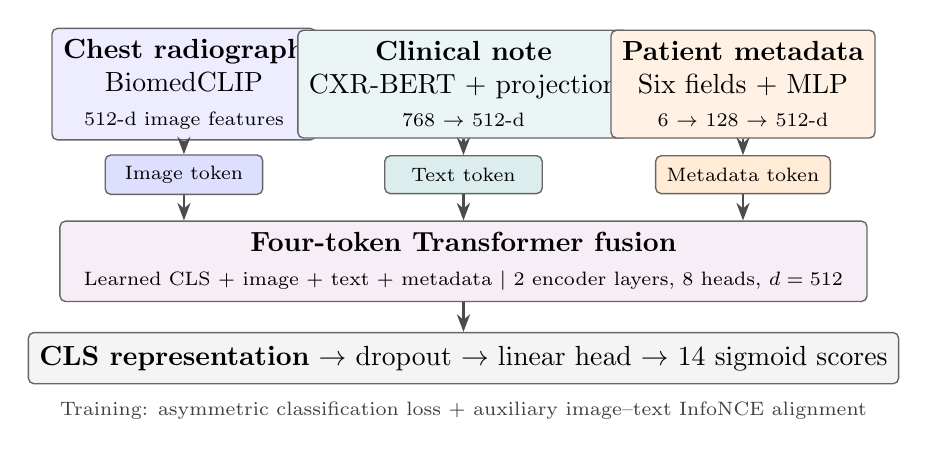
\begin{tikzpicture}[x=1cm,y=1cm,>=Stealth,
 box/.style={draw=black!60,rounded corners=2pt,line width=.5pt,align=center,inner sep=4pt},
 arrow/.style={->,line width=.75pt,draw=black!70},
 label/.style={font=\scriptsize,align=center}]
% Modality-specific encoders
\node[box,fill=blue!7,minimum width=3.15cm,minimum height=1.18cm] (vis) at (1.7,4.1)
 {\textbf{Chest radiograph}\\BiomedCLIP\\\scriptsize 512-d image features};
\node[box,fill=teal!8,minimum width=3.15cm,minimum height=1.18cm] (txt) at (5.25,4.1)
 {\textbf{Clinical note}\\CXR-BERT + projection\\\scriptsize 768 $\rightarrow$ 512-d};
\node[box,fill=orange!10,minimum width=3.15cm,minimum height=1.18cm] (met) at (8.8,4.1)
 {\textbf{Patient metadata}\\Six fields + MLP\\\scriptsize 6 $\rightarrow$ 128 $\rightarrow$ 512-d};
% tokens
\node[box,fill=blue!13,minimum width=2.0cm,minimum height=.48cm,font=\scriptsize] (vt) at (1.7,2.95) {Image token};
\node[box,fill=teal!14,minimum width=2.0cm,minimum height=.48cm,font=\scriptsize] (tt) at (5.25,2.95) {Text token};
\node[box,fill=orange!16,minimum width=2.0cm,minimum height=.48cm,font=\scriptsize] (mt) at (8.8,2.95) {Metadata token};
\draw[arrow] (vis.south)--(vt.north);\draw[arrow] (txt.south)--(tt.north);\draw[arrow] (met.south)--(mt.north);
% Fusion
\node[box,fill=violet!7,minimum width=10.25cm,minimum height=1.02cm] (fusion) at (5.25,1.85)
 {\textbf{Four-token Transformer fusion}\\\scriptsize Learned CLS + image + text + metadata $\mid$ 2 encoder layers, 8 heads, $d=512$};
\draw[arrow] (vt.south) -- (vt.south |- fusion.north);
\draw[arrow] (tt.south) -- (tt.south |- fusion.north);
\draw[arrow] (mt.south) -- (mt.south |- fusion.north);
\node[box,fill=gray!9,minimum width=7.1cm,minimum height=.65cm] (head) at (5.25,.62)
 {\textbf{CLS representation} $\rightarrow$ dropout $\rightarrow$ linear head $\rightarrow$ 14 sigmoid scores};
\draw[arrow] (fusion.south)--(head.north);
\node[label,text=black!75] at (5.25,-.05) {Training: asymmetric classification loss + auxiliary image--text InfoNCE alignment};
\end{tikzpicture}
}
\caption{X-Fusion architecture. Three modality-specific encoders produce 512-d tokens that join a learned CLS token in a two-layer Transformer. The classifier predicts fourteen finding scores. Visual attention and metadata-attribution displays are produced separately by the inference interface.}
\label{fig:architecture}
\end{figure}

\subsection{Optimization Objectives}

Let $p_{ik}$ denote the predicted probability for finding $k$ in sample $i$, and $y_{ik}\!\in\!\{0,1\}$ its label.
With margin shift $\delta\!=\!0.05$ and $q_{ik}\!=\!\min(1-p_{ik}+\delta,\,1)$, the Asymmetric Loss per label is:

\begin{multline}
\ell_{ik}=
-y_{ik}(1-p_{ik})
\log(\max(p_{ik},\epsilon))\\
-(1-y_{ik})(1-q_{ik})^4
\log(\max(q_{ik},\epsilon)),
\end{multline}

\noindent where $\epsilon\!=\!10^{-8}$.
The batch-averaged classification loss is $\mathcal{L}_{\mathrm{ASL}}\!=\!B^{-1}\!\sum_{i,k}\ell_{ik}$.

For $\ell_2$-normalized image and text features $v_i,t_j$, the similarity matrix is $C_{ij}\!=\!v_i^\top t_j/\tau$ with temperature $\tau\!=\!0.07$.
The symmetric contrastive alignment loss is:

\begin{align}
\mathcal{L}_{\mathrm{NCE}}
&=\tfrac{1}{2}
[\operatorname{CE}(C,a)+
\operatorname{CE}(C^\top\!,a)],\\
\mathcal{L}_{\mathrm{train}}
&=\mathcal{L}_{\mathrm{ASL}}
+0.1\,\mathcal{L}_{\mathrm{NCE}},
\end{align}

\noindent where $a$ contains matching in-batch image--text indices.

% =================================================================
% 4. DATASET AND EXPERIMENTAL SETUP
% =================================================================
\section{Dataset and Experimental Setup}

\subsection{Data Partitioning}

The study uses 31{,}630 images matched from 31{,}877 available PNG files in a local subset of NIH ChestX-ray14~\cite{nihdataset}.
The official \texttt{train\_val\_list.txt} and \texttt{test\_list.txt} define the split boundary.
The training/validation pool is further divided by patient ID (seed 42, 10\% validation).
Table~\ref{tab:split} and Table~\ref{tab:prevalence} summarize the partition statistics.

Images are resized to $224\!\times\!224$ pixels, converted to RGB, and normalized with ImageNet channel statistics.
Training augmentation applies horizontal flips, rotations ($\leq\!10^\circ$), and brightness/contrast jitter (0.15).
Test preprocessing is deterministic.

\begin{table}[t]
\caption{Patient-disjoint dataset partitions. No patient ID overlap exists across splits.}
\label{tab:split}
\centering\small
\begin{tabular}{lrr}
\toprule
Partition & Images & Patients\\
\midrule
Training & 21{,}964 & 9{,}939\\
Validation & 2{,}566 & 1{,}104\\
Test & 7{,}100 & 1{,}137\\
\midrule
Total & 31{,}630 & 12{,}180\\
\bottomrule
\end{tabular}
\end{table}

\begin{table}[t]
\caption{Positive-label counts by partition. Pneumonia (18 test positives) and Consolidation (62) are extremely rare.}
\label{tab:prevalence}
\centering\small
\begin{tabular}{lrrr}
\toprule
Finding & Train & Val & Test\\
\midrule
Atelectasis & 3{,}237 & 367 & 879\\
Cardiomegaly & 723 & 107 & 387\\
Effusion & 2{,}687 & 329 & 1{,}270\\
Infiltration & 3{,}629 & 433 & 1{,}128\\
Mass & 1{,}600 & 164 & 476\\
Nodule & 2{,}111 & 226 & 476\\
Pneumonia & 42 & 5 & 18\\
Pneumothorax & 1{,}148 & 131 & 1{,}024\\
Consolidation & 132 & 11 & 62\\
Edema & 395 & 43 & 262\\
Emphysema & 557 & 70 & 335\\
Fibrosis & 558 & 57 & 190\\
Pleural Thick. & 787 & 94 & 348\\
Hernia & 63 & 8 & 49\\
\bottomrule
\end{tabular}
\end{table}

\subsection{Auxiliary Input Construction and Training Configuration}

Age and sex are extracted from the original NIH CSV metadata.
In the current implementation, clinical-note text is generated from disease-label templates, and four vital signs (temperature, heart rate, respiratory rate, SpO$_2$) are sampled from Gaussian distributions conditioned on the presence of Pneumonia or Edema.
This creates a direct information pathway from target labels to predictors---the core evaluation integrity issue analyzed in Section~5.

Training uses AdamW ($\text{lr}\!=\!2\!\times\!10^{-4}$, weight decay $10^{-4}$), cosine annealing, batch size 4 with 8-step gradient accumulation (effective batch 32), 16-bit mixed precision, and a frozen text encoder.
The available checkpoint corresponds to epoch 14 of a 15-epoch schedule.

% =================================================================
% 5. RESULTS AND ANALYSIS
% =================================================================
\section{Results and Analysis}

\subsection{Optimization Records}

Fourteen logged epochs show the training objective (ASL + 0.1$\cdot$InfoNCE) decreasing from 0.1545 to 0.1190 (22.95\% relative reduction), and validation ASL decreasing from 0.0207 to 0.0007.
Training and validation track different objectives; their scales are not directly comparable.
Fig.~\ref{fig:losses} shows the optimization traces.
These curves document convergence of the configured objective, not independent diagnostic performance.

\begin{figure}[t]
\centering
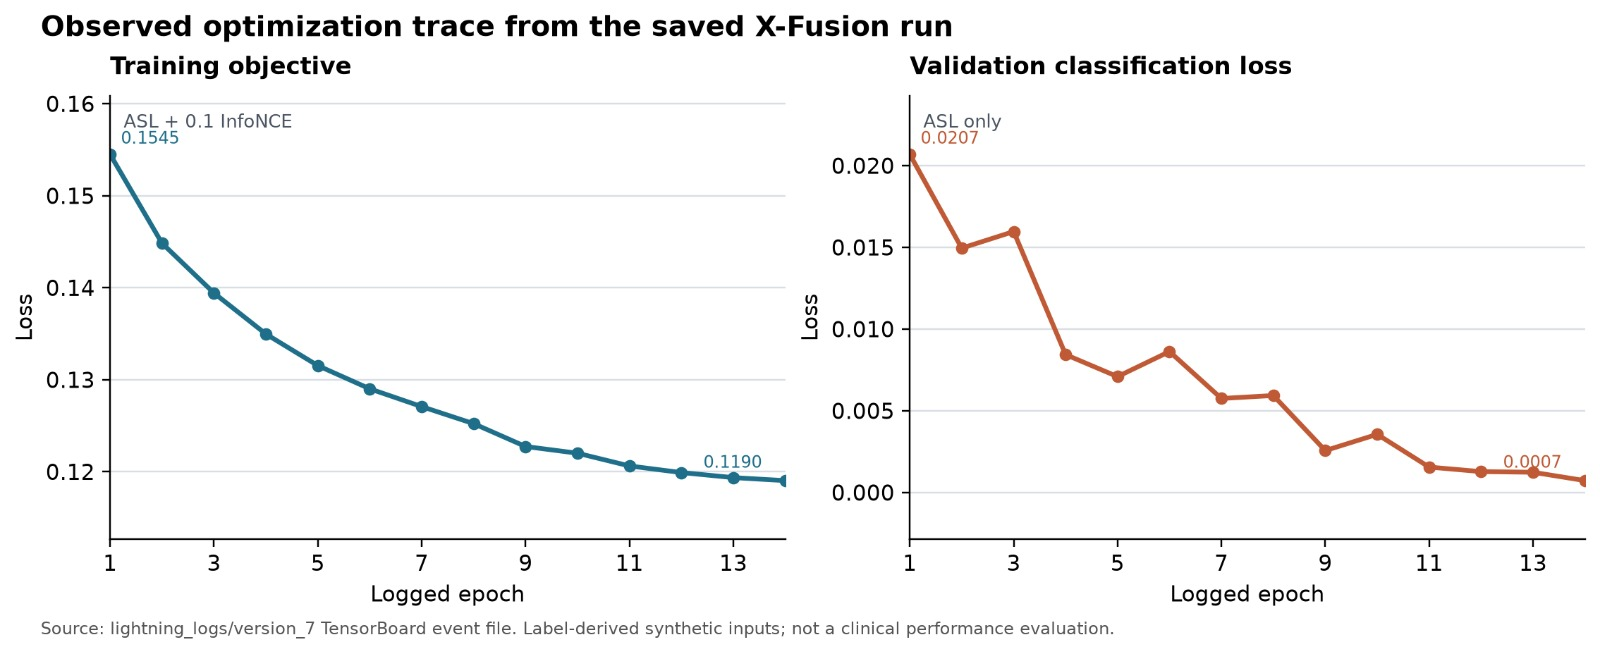
\includegraphics[width=\linewidth]{optimization_traces.jpg}
\caption{Optimization traces for fourteen epochs. Training objective includes contrastive regularization; validation uses ASL only. Both operate on label-conditioned auxiliary inputs.}
\label{fig:losses}
\end{figure}

\subsection{Recomputed Software Diagnostics}

The saved prediction file contains 7{,}100 distinct image identifiers with fourteen binary targets and fourteen probability columns.
We recomputed metrics from these saved outputs: AUROC via empirical ROC integration, average precision via recall-weighted precision sums, and F1 from pooled confusion counts at threshold 0.5.
Table~\ref{tab:diagnostics} reports the results.

\begin{table}[t]
\caption{Recomputed diagnostics from saved predictions. These values are inflated by label-conditioned auxiliary inputs and do not constitute clinical performance estimates.}
\label{tab:diagnostics}
\centering
\begin{tabular}{lr}
\toprule
Metric & Value\\
\midrule
Macro AUROC & 0.9999\\
Macro average precision & 0.9953\\
Macro F1 (threshold 0.5) & 0.9709\\
Pneumonia precision (0.5) & 0.5667\\
Pneumonia recall (0.5) & 0.9444\\
Pneumonia F1 (0.5) & 0.7083\\
\bottomrule
\end{tabular}
\end{table}

\subsection{Evaluation Integrity Diagnosis}
\label{sec:integrity}

The near-perfect macro scores are a direct consequence of input construction.
The report generator selects disease-specific text templates using the target label list; a model with access to these notes can recover the labels without examining the radiograph.
Similarly, the metadata generator samples physiological values from distributions whose parameters change based on Pneumonia or Edema presence.
This constitutes \emph{target leakage}: test-case inputs carry target-derived information.

Patient-disjoint splitting prevents image-level or patient-level data leakage between partitions.
However, it cannot remedy the within-case dependency where each individual test sample's auxiliary inputs are constructed from its own labels.
Consequently, no component of the multimodal performance can be attributed to independently observed clinical context.

For Pneumonia specifically, the saved predictions yield TP\,=\,17, FP\,=\,13, FN\,=\,1 at threshold 0.5 among 18 positives and 7{,}082 negatives.
This illustrates how high aggregate ranking scores can coexist with modest precision on extremely rare labels.

\subsection{Independent-Input Reference Experiment}
\label{sec:baselines}

To establish reproducible reference evidence free from auxiliary-input contamination, we trained new models using only independently observed predictors.
Four configurations were evaluated:

\begin{itemize}
\item \textbf{Training prevalence}: constant per-label prediction using training-set label frequencies (chance-level reference).
\item \textbf{Age + sex}: two recorded demographic features from the NIH CSV.
\item \textbf{Image pixels}: 16$\times$16 grayscale-resized images (256 pixel features scaled to $[0,1]$).
\item \textbf{Pixels + age/sex}: combined 258-feature input.
\end{itemize}

All non-trivial models use fourteen independent L2-regularized logistic regressions with L-BFGS, regularization strength $C\!\in\!\{0.01, 0.1, 1\}$ selected by validation macro AUROC, seed 42, and at most 500 iterations (all models converged).
Age values outside $[0,120]$ are imputed with the training median (51.0).
Missing gender is encoded as 0.5.
All standardization is fitted on training data only.
\textbf{No predictor is derived from any disease label.}

Table~\ref{tab:independent} reports held-out test scores, and Table~\ref{tab:perlabel} provides per-label detail for the combined model.

\begin{table}[t]
\caption{Independent-input reference experiment on 7{,}100 test images. These linear models provide reproducible, leakage-free baselines. They do not validate the tri-modal Transformer.}
\label{tab:independent}
\centering\small
\begin{tabular}{lrrr}
\toprule
Configuration & Macro AUROC & Macro AP & Macro F1\\
\midrule
Training prevalence & 0.5000 & 0.0695 & 0.0000\\
Age + sex ($C\!=\!0.1$) & 0.5518 & 0.0861 & 0.0000\\
Image pixels ($C\!=\!0.01$) & 0.6317 & 0.1178 & 0.0098\\
Pixels + age/sex ($C\!=\!0.01$) & \textbf{0.6344} & \textbf{0.1201} & \textbf{0.0106}\\
\bottomrule
\end{tabular}
\end{table}

\begin{table}[t]
\caption{Per-label AUROC for the combined pixels + age/sex reference model (7{,}100 test images). Best-performing labels tend to have higher prevalence or distinct morphological signatures.}
\label{tab:perlabel}
\centering\small
\begin{tabular}{lrr}
\toprule
Finding & AUROC & Test positives\\
\midrule
Atelectasis & 0.640 & 879\\
Cardiomegaly & 0.749 & 387\\
Effusion & 0.684 & 1{,}270\\
Infiltration & 0.595 & 1{,}128\\
Mass & 0.575 & 476\\
Nodule & 0.633 & 476\\
Pneumonia & 0.516 & 18\\
Pneumothorax & 0.646 & 1{,}024\\
Consolidation & 0.478 & 62\\
Edema & 0.718 & 262\\
Emphysema & 0.552 & 335\\
Fibrosis & 0.757 & 190\\
Pleural Thick. & 0.563 & 348\\
Hernia & 0.777 & 49\\
\bottomrule
\end{tabular}
\end{table}

These reference models are deliberately simple linear classifiers on low-resolution features.
Their purpose is not to match pretrained deep encoders but to establish a reproducible, uncontaminated measurement floor.
Comparing the contaminated X-Fusion scores (macro AUROC $\approx$~1.0) directly to these baselines would change both the input space and model family simultaneously---such a comparison does not isolate a fusion effect.

\subsection{Explanation Views and Application Interface}

The inference interface provides two explanation modalities.
\textbf{Visual attention}: the final Transformer block's CLS-to-patch attention weights are averaged across heads, reshaped to a $14\!\times\!14$ grid, upsampled, and overlaid on the input image.
This is an attention visualization, not Chefer relevance propagation~\cite{chefer2021} or validated lesion localization.
\textbf{Metadata attribution}: Kernel SHAP~\cite{lundberg2017} perturbs the six metadata fields while holding image and text features fixed.
Absolute contributions are aggregated across outputs and normalized, which removes sign and finding specificity.

A Next.js frontend communicates with a FastAPI inference service.
The interface accepts a radiograph, clinical text, and structured fields, returning finding scores with explanation views.
These implement a demonstration workflow and have not been clinically calibrated.

% =================================================================
% 6. LIMITATIONS AND FUTURE DIRECTIONS
% =================================================================
\section{Limitations and Future Directions}

The primary limitation is target leakage through generated notes and label-conditioned vital signs, which prevents clinical-performance interpretation of the tri-modal scores.
Additional limitations include:

\begin{itemize}
\item Weak image-level labels from automated NLP extraction~\cite{wang2017}, not expert annotation.
\item Evaluation on a subset (31{,}630 of 112{,}120 images) of a single dataset.
\item Extremely few positive cases for Pneumonia (18 test) and Consolidation (62 test).
\item Uncalibrated decision thresholds not validated on independent clinical data.
\item Unvalidated explanation fidelity for both attention overlays and SHAP attributions.
\end{itemize}

\textbf{Required future work.}
(1)~Acquire auxiliary inputs (clinical notes, vital signs) recorded independently of the target diagnosis, such as from MIMIC-CXR linked with MIMIC-IV clinical data.
(2)~Retrain the tri-modal model with corrected inputs; changing test inputs alone introduces distribution shift without repairing training contamination.
(3)~Conduct matched ablations (image-only, image+text, image+metadata, full fusion) under identical training budgets and evaluation protocols.
(4)~Select class-specific thresholds on validation data and evaluate the held-out test set once.
(5)~Report calibration curves, patient-level uncertainty, and external-dataset generalization.
(6)~Validate explanation fidelity through quantitative localization benchmarks.

% =================================================================
% 7. CONCLUSION
% =================================================================
\section{Conclusion}

X-Fusion demonstrates a compact Transformer-based integration of pretrained visual and language encoders with structured patient metadata for fourteen-label chest radiograph analysis, connected to an explanation-enabled web interface.
The system's implementation is fully functional and its training records document stable optimization convergence.
However, our systematic analysis reveals that label-conditioned auxiliary inputs create within-case target leakage that patient-disjoint splitting cannot remedy, rendering the near-perfect evaluation scores uninformative about clinical discrimination.
The newly contributed independent-input reference experiment establishes leakage-free baselines (macro AUROC 0.634) using only real image pixels and recorded demographics.
This work underscores that \emph{evaluation integrity verification}---confirming that every predictor is collected independently of the reference standard---is a necessary step before multimodal medical AI systems can claim clinical benefit.

\subsubsection{Disclosure.}
AI-assisted tools were used for manuscript drafting, equation formatting, and code review.
This disclosure does not attribute authorship to any tool or establish the validity of experiments.

\bibliographystyle{splncs04}
\bibliography{references}

\end{document}
